\section*{1D 系統架構}

\subsection*{設計理念}

我們以鋼球平衡台作為專題的主體,然後寫程式驅動雷射測距感測器當鋼球遠離時platform,當鋼球靠近時platform放下,重複此動作直至鋼球平衡台平衡。

\begin{figure}[h!]
    \centering
    \begin{minipage}[b]{0.45\textwidth}
        \centering
        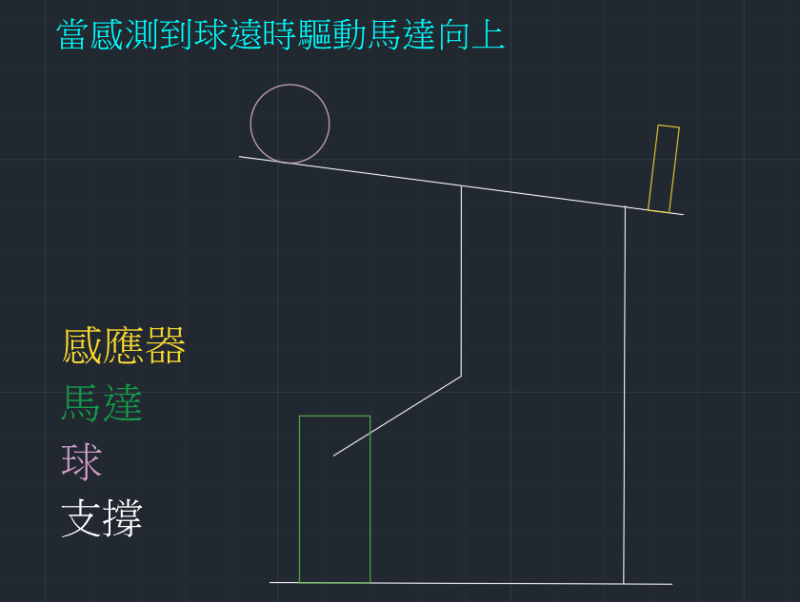
\includegraphics[width=\textwidth,height=0.2\textheight]{./../images/螢幕擷取畫面 2024-05-22 181158.png}
        \caption{2D草圖(1)}
    \end{minipage}
    \hfill
    \begin{minipage}[b]{0.45\textwidth}
        \centering
        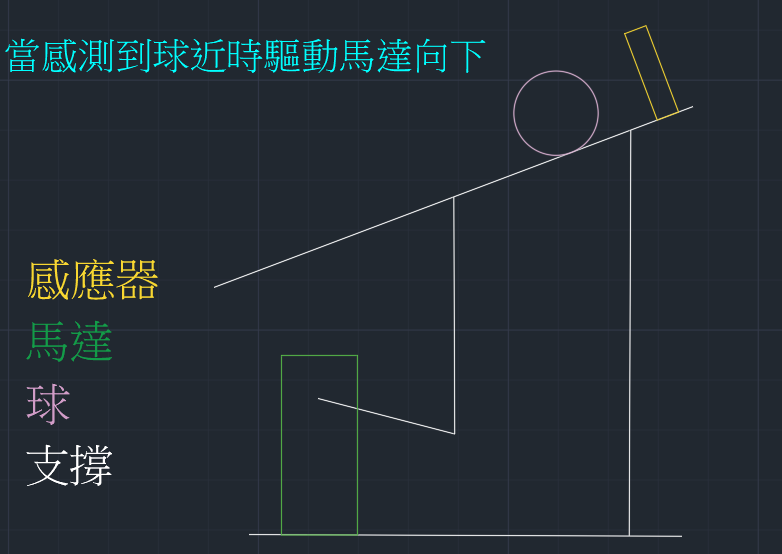
\includegraphics[width=\textwidth,height=0.2\textheight]{./../images/螢幕擷取畫面 2024-05-22 180925.png} 
        \caption{2D草圖(2)}
    \end{minipage}
\end{figure}

專題使用\textbf{solidwork 2023}進行繪圖

\begin{figure}[h!]
    \centering
    
\includegraphics[width=0.5\textwidth]{./../images/6-1-1.png}
    \caption{SOLIDWORKS}
\end{figure}

\noindent SOLIDWORKS是一款用於設計各種產品和零件。 模擬和分析: 提供模擬和分析工具,用於測試設計的性能、耐久性和材料屬性。 製造和加工: 支援數控機床編程和工具路徑生成,提高製造效率。 綜合性: 提供組件建模、裝配設計、繪圖生成、動態模擬、流體動力學模擬等多個功能。

\noindent 預計會使用的功能有


\subsection{platform}
第一版本鋼球平衡台的\textbf{platform}軌道長度為\textbf{200mm}整體的寬度為\textbf{30mm} 並給定深度填料\textbf{11mm}

\begin{figure}[h!]
    \centering
    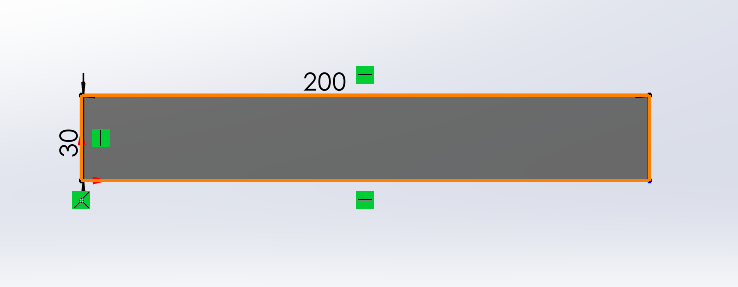
\includegraphics[width=0.8\textwidth]{./../images/6-1-11.png}
    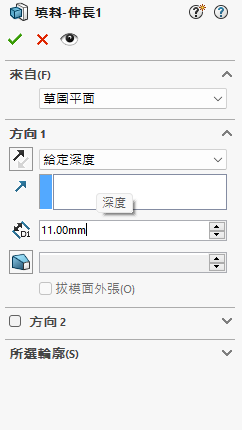
\includegraphics[width=0.2\textwidth]{./../images/6-1-12.png}
\end{figure}

\noindent 軌道上方寬度為\textbf{8.5mm}下方為\textbf{7.2mm}深\textbf{4mm}並將紅圈處深伸長除料選擇完全貫穿

\begin{figure}[h!]
    \centering
    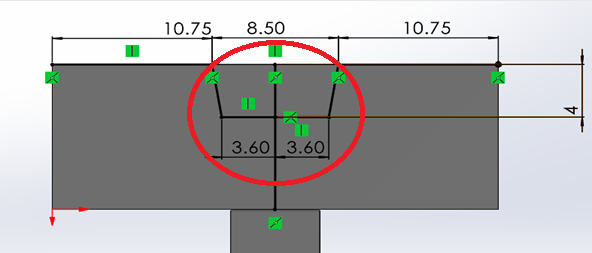
\includegraphics[width=0.8\textwidth]{./../images/6-1-13.png}
    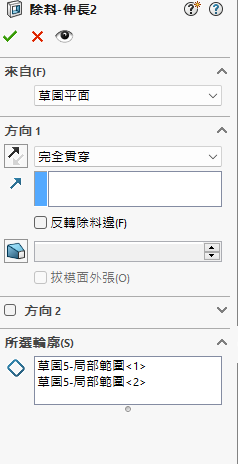
\includegraphics[width=0.2\textwidth]{./../images/6-1-14.png}
\end{figure}

\noindent 下方配合處長\textbf{30mm}寬\textbf{6mm} 繪製好圖形草圖

\begin{figure}[h!]
    \centering
    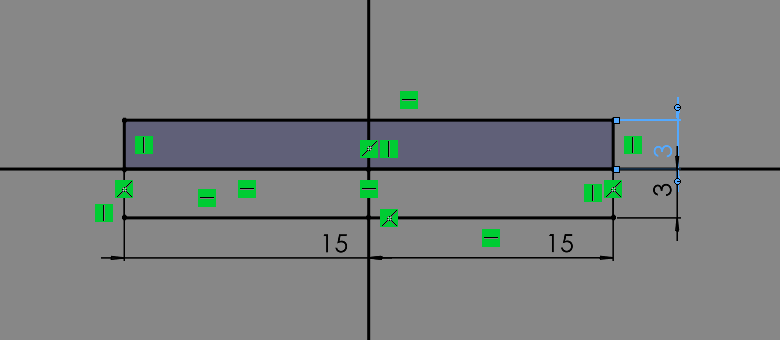
\includegraphics[width=1\textwidth]{./../images/6-1-15.png}
\end{figure}

\noindent 給予尺寸後伸長填料\textbf{25mm}

\begin{figure}[h!]
    \centering
    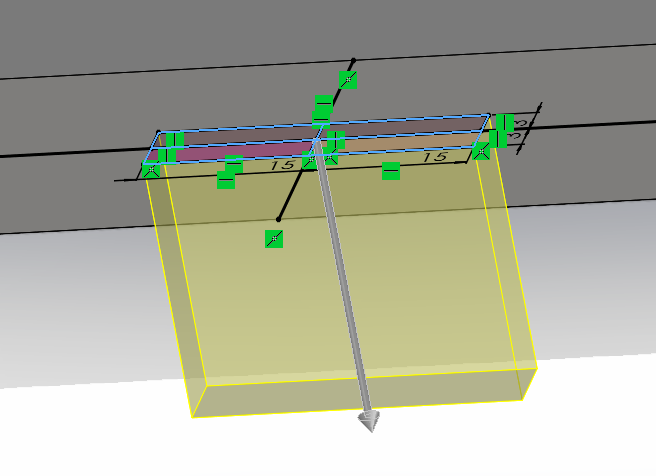
\includegraphics[width=0.6\textwidth]{./../images/6-1-16.png}
    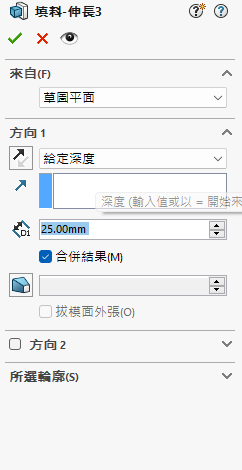
\includegraphics[width=0.2\textwidth]{./../images/6-1-17.png}
\end{figure}

\noindent 填料完成後再圖形上畫一個\textbf{2.9mm}的小孔並進行伸長除料以便與其他零件配合

\begin{figure}[h!]
    \centering
    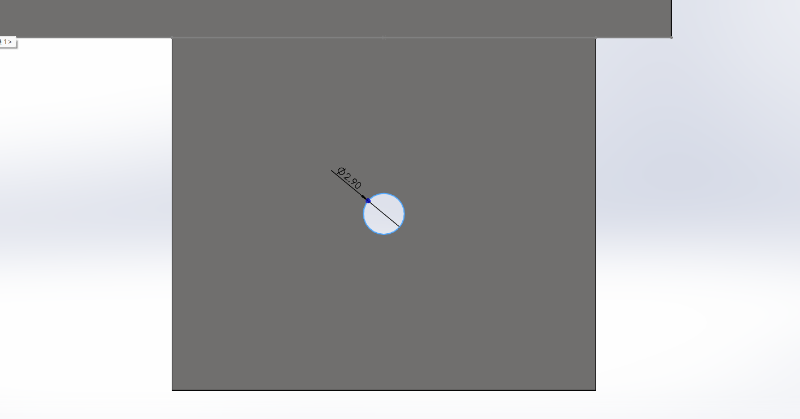
\includegraphics[width=1\textwidth]{./../images/6-1-18.png}
\end{figure}

\noindent 第一版\textbf{platform}完成圖

\begin{figure}[h!]
    \centering
    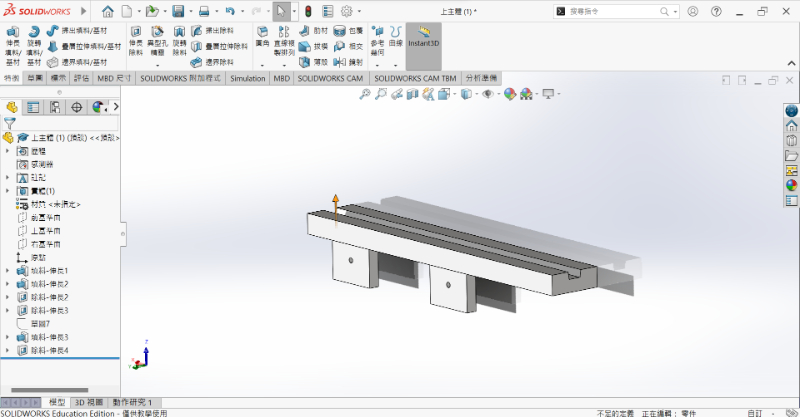
\includegraphics[width=1\textwidth]{./../images/6-1-19.png}
\end{figure}

\noindent 修改部分

\noindent 軌道上方增加長\textbf{26.2mm}寬\textbf{2mm}的貫穿凹槽,用於放置感應器

\begin{figure}[h!]
    \centering
    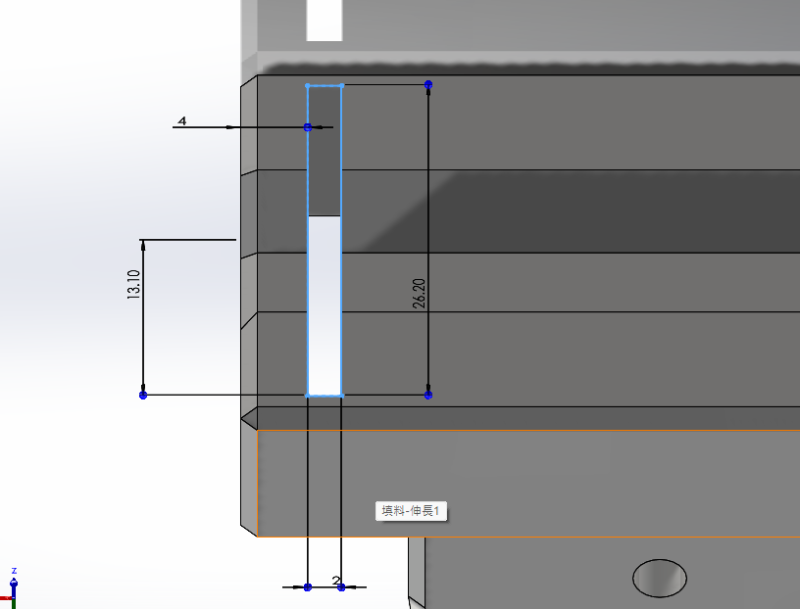
\includegraphics[width=1\textwidth]{./../images/6-1-20.png}
\end{figure}

\noindent 下方接合處新增\textbf{R10}圓角

\begin{figure}[h!]
    \centering
    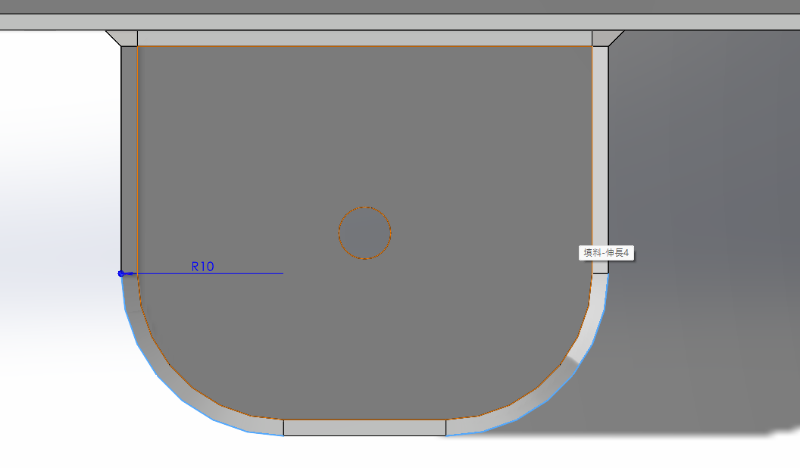
\includegraphics[width=1\textwidth]{./../images/6-1-21.png}
\end{figure}

\noindent 最終Platform零件圖

\begin{figure}[h!]
    \centering
    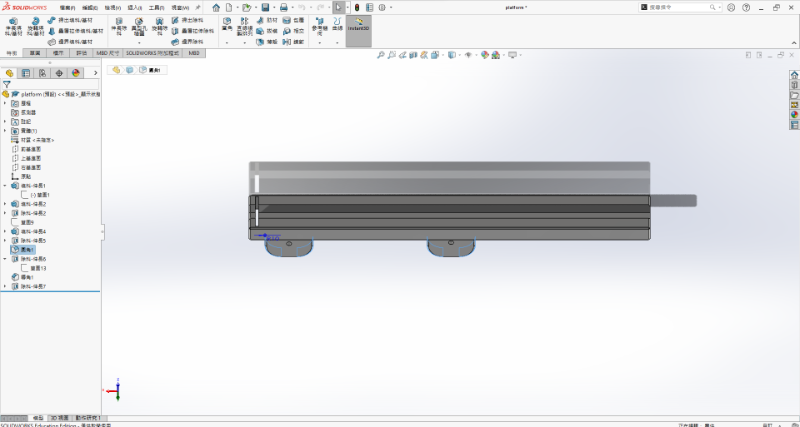
\includegraphics[width=1\textwidth]{./../images/6-1-22.png}
\end{figure}

\noindent 3D列印成果

\begin{figure}[h!]
    \centering
    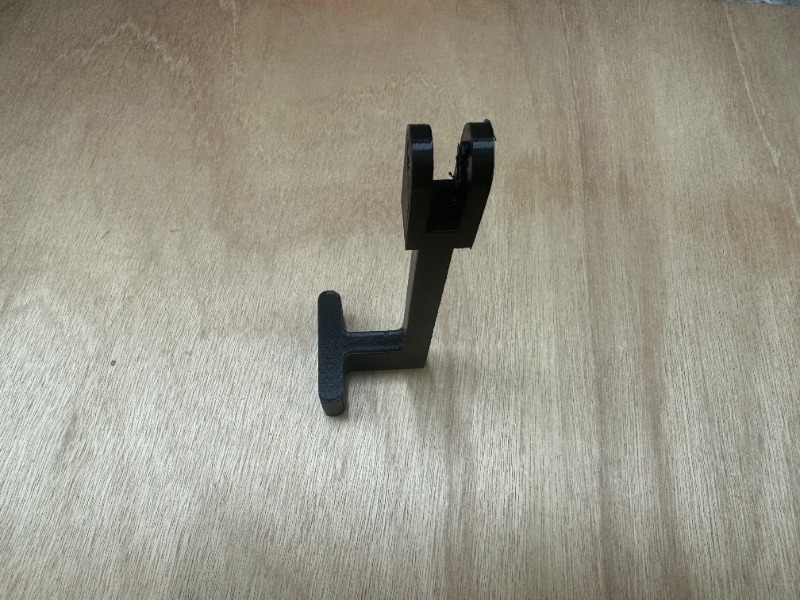
\includegraphics[width=0.5\textwidth]{./../images/6-1-24.JPG}
\end{figure}

\subsection{base}
第一版\textbf{Base}底的長為\textbf{237mm}寬為\textbf{150mm}

\begin{figure}[h!]
    \centering
    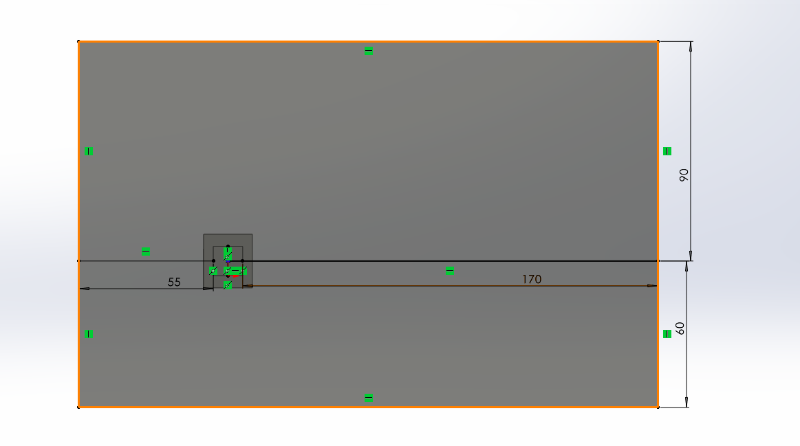
\includegraphics[width=1\textwidth]{./../images/6-1-27.png}
\end{figure}

\noindent 在底板長\textbf{55mm}寬\textbf{54mm}處繪製一個\textbf{12mmX12mm}的方形柱並向上填料\textbf{100mm}

\begin{figure}[h!]
    \centering
    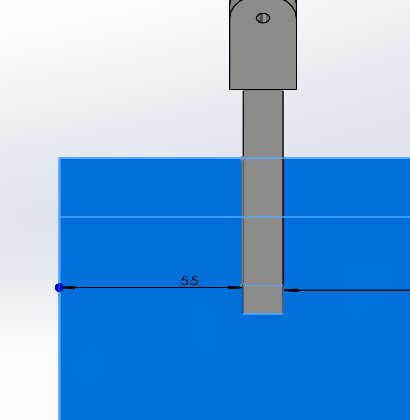
\includegraphics[width=0.5\textwidth]{./../images/6-1-28.png}
    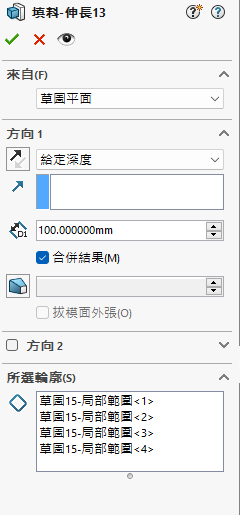
\includegraphics[width=0.2\textwidth]{./../images/6-1-29.png}
\end{figure}

\noindent 在方柱上方繪製一個長30.28mm寬\textbf{20}的長方體然後在長方體上畫直徑20mm的半圓最後在圓的中心繪製一個3.98mm的小孔最後在長方體上畫一個長30mm寬10.8mm的小長方體伸長除料選擇完全貫穿方便與上方platform配合

\begin{figure}[h!]
    \centering
    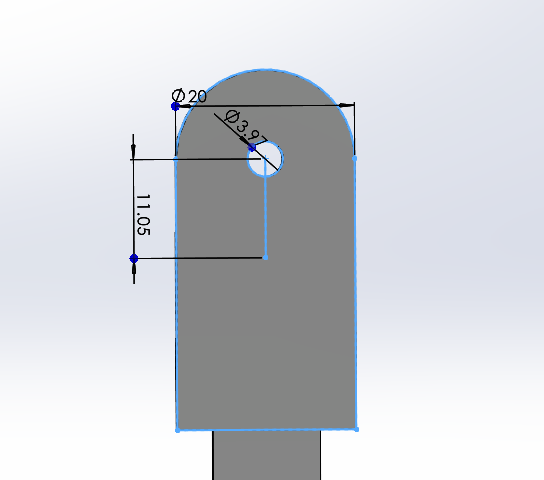
\includegraphics[width=0.3\textwidth]{./../images/6-1-30.png}
    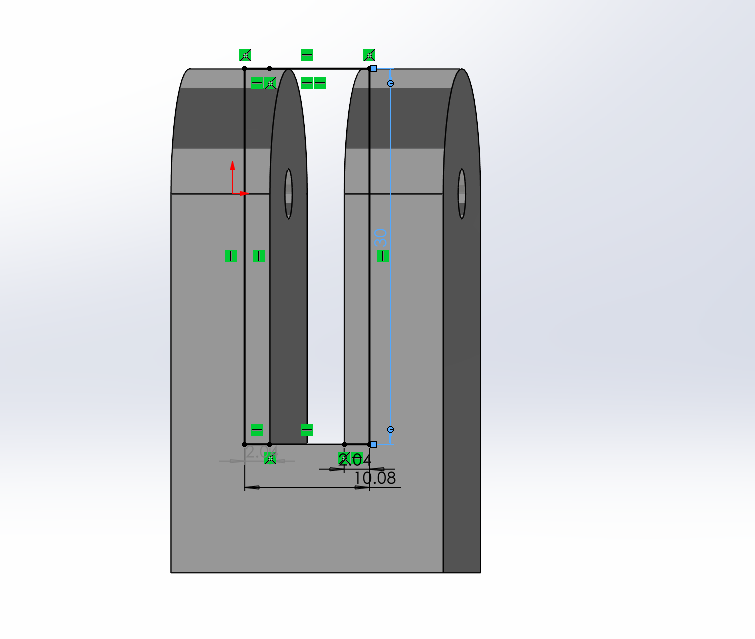
\includegraphics[width=0.3\textwidth]{./../images/6-1-31.png}
    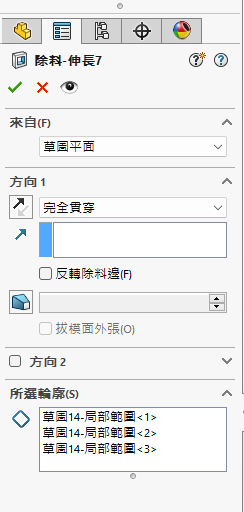
\includegraphics[width=0.1\textwidth]{./../images/6-1-32.png}
\end{figure}

\noindent 在距離方柱中心長\textbf{129mm}寬\textbf{25mm}處繪製一個長\textbf{31mm}寬\textbf{20mm}向上填料\textbf{7mm}的小平台用來定位馬達

\begin{figure}[h!]
    \centering
    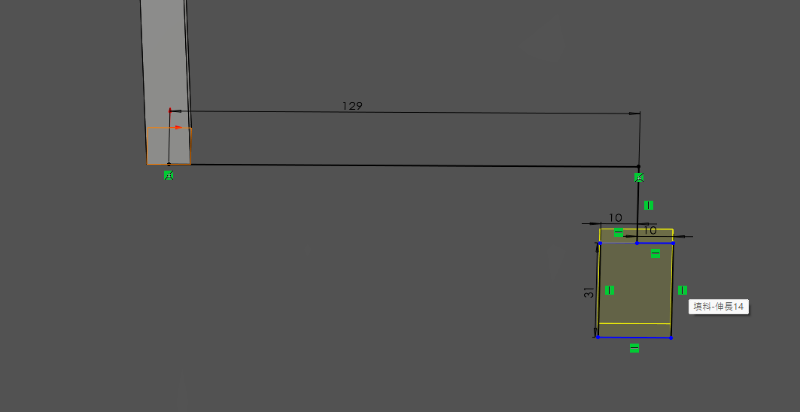
\includegraphics[width=0.5\textwidth]{./../images/6-1-33.png}
    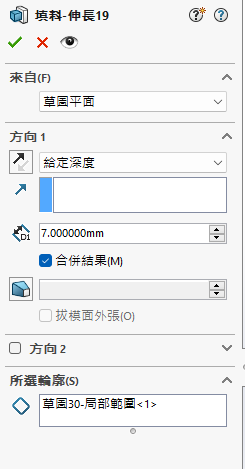
\includegraphics[width=0.2\textwidth]{./../images/6-1-34.png}
\end{figure}

\noindent 並且在兩邊加畫底\textbf{15mm}高\textbf{45mm}的三角形支撐架防止馬達晃動

\begin{figure}[h!]
    \centering
    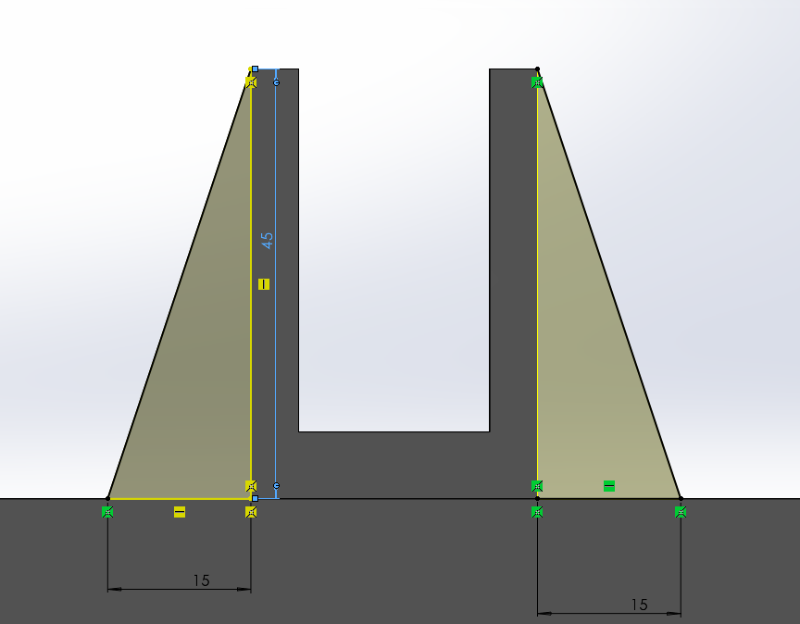
\includegraphics[width=0.6\textwidth]{./../images/6-1-35.png}
\end{figure}

\noindent 第一版base完成圖

\begin{figure}[h!]
    \centering
    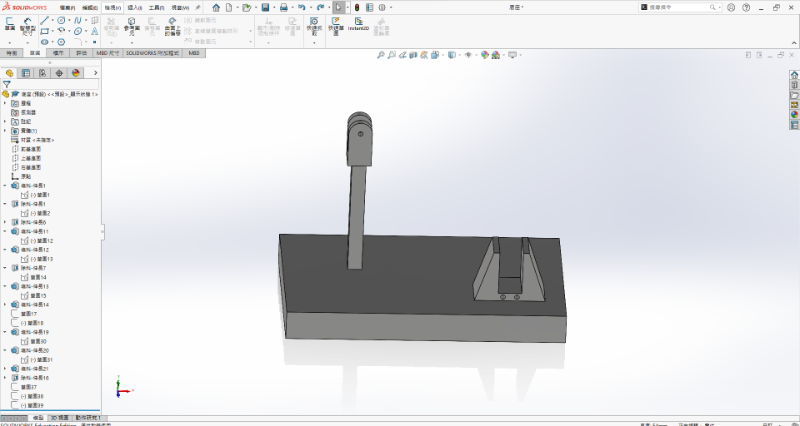
\includegraphics[width=1\textwidth]{./../images/6-1-36.png}
\end{figure}

\noindent 修改部分

\noindent 底部去除浪費的部分改以長165.6mm圓直徑22.35mm的直狹槽代替

\begin{figure}[h!]
    \centering
    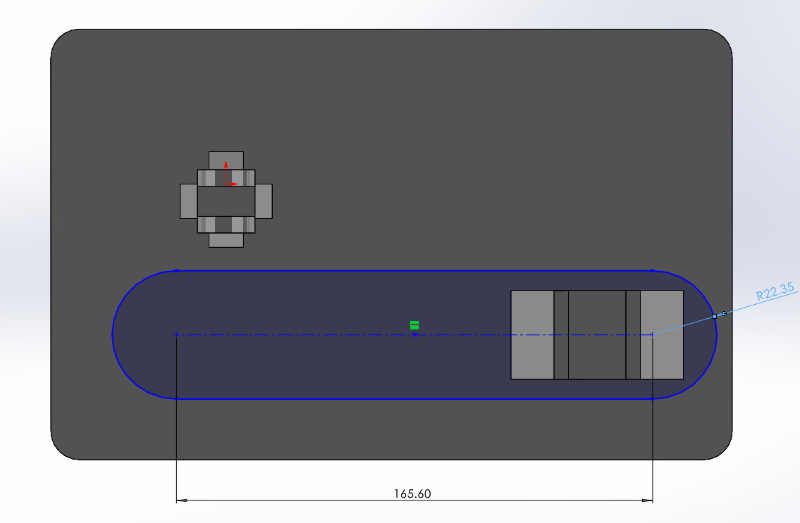
\includegraphics[width=1\textwidth]{./../images/6-1-37.png}
\end{figure}

\noindent 為了好收納將左方柱子拔除留下一凹槽方便後續配合及螺絲孔

\begin{figure}[h!]
    \centering
    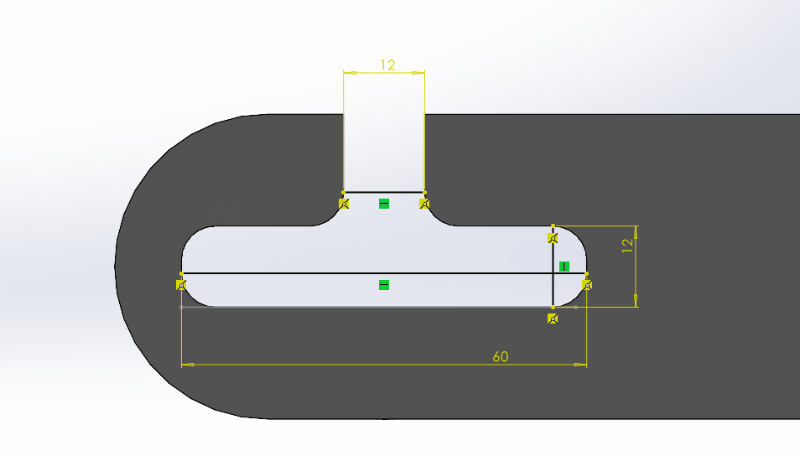
\includegraphics[width=1\textwidth]{./../images/6-1-38.png}
\end{figure}

\noindent 最終base完成圖

\begin{figure}[h!]
    \centering
    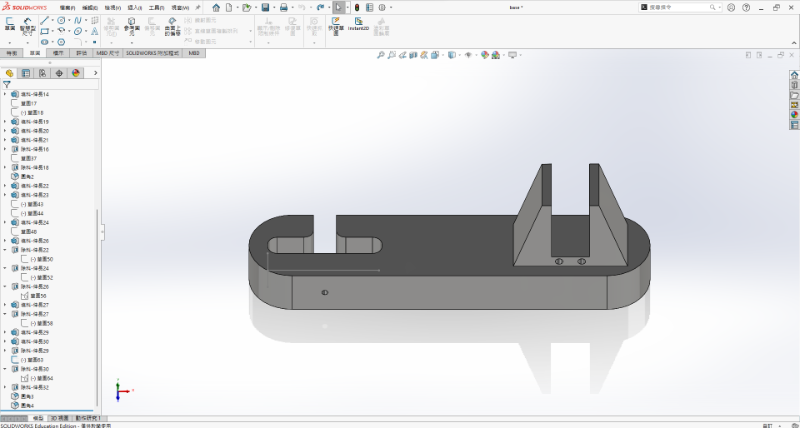
\includegraphics[width=1\textwidth]{./../images/6-1-39.png}
\end{figure}

\noindent 3D列印成果

\begin{figure}[h!]
    \centering
    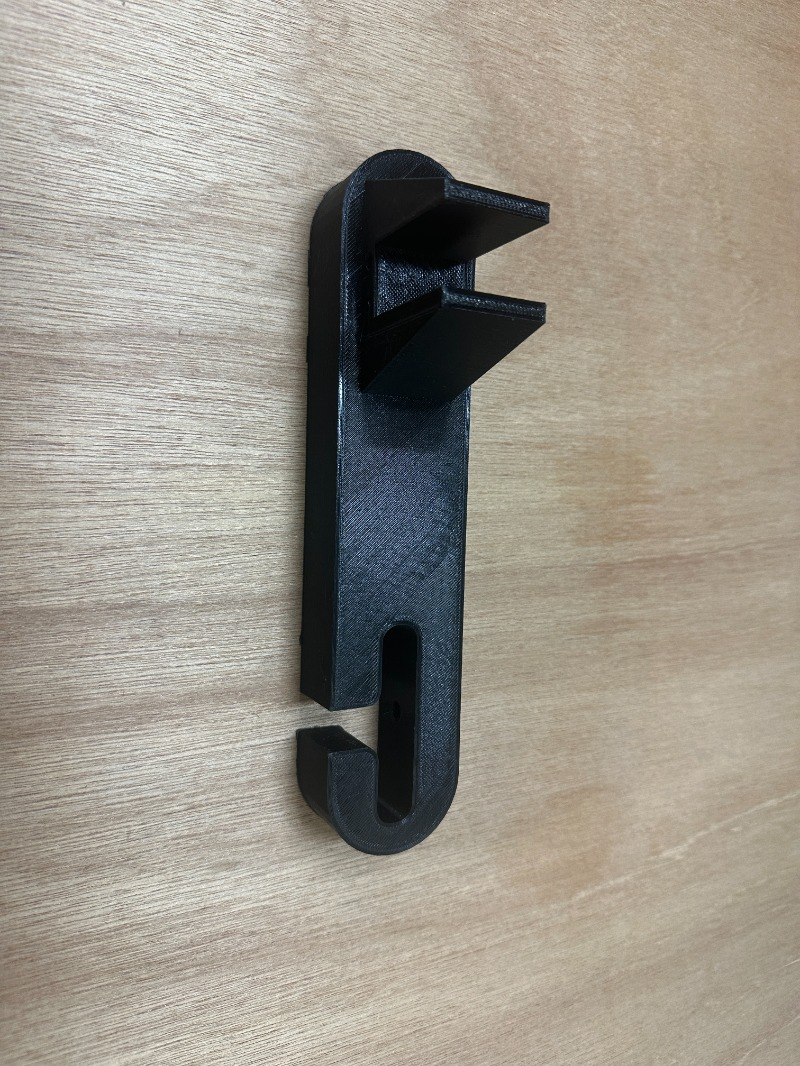
\includegraphics[width=0.5\textwidth]{./../images/6-1-25.JPG}
\end{figure}


